\subsection{Asymmetric Interconnect Management}
\label{interconnect}

Dynamic NVLink balancing Is there any space for improvement? The idea is to turn 
around sub-channels which are not utilized. 

Graph 0: We need a stacked-bar graph that shows what’s the percentage of total 
exe time spent in configs where: both directions are saturated (no room for 
improvement), only one direction is saturated (here we can improve), none is 
saturated (we don’t care for this). Do we want to show this as aggregate number 
of per-GPU?
We explain the algorithm how and when we increment and decrement the number of 
sub-channels per direction. Two important parameters: link switch time and 
sample time.

Graph 1: baseline is 1x NVLink, upper bound is 2x NVLink, link switch time is 
100 cycles, we show the speedup for different sample time values (1K, 2K, 5K, 
10K, 100K cycles). Finner measurements are better.

Graph 2a: baseline is 1x NVLink, upper bound is 2x NVLink, sample\_time is 1K. 
We swipe through link\_switch\_time (10, 100, 200, 500 cycles). Here, link 
switch time is important, we want it to be low.

Graph 2b: the same, but sample\_time is 100K. Here, we do not care about link 
switch time. The point where it starts to matter is 5K (or 2K) cycles and below. 
From now on, we assume 100 cycles for link switch time and 5K (or 2K) cycles for 
sampling period.

\begin{figure}[tp]
    \centering
<<<<<<< HEAD
    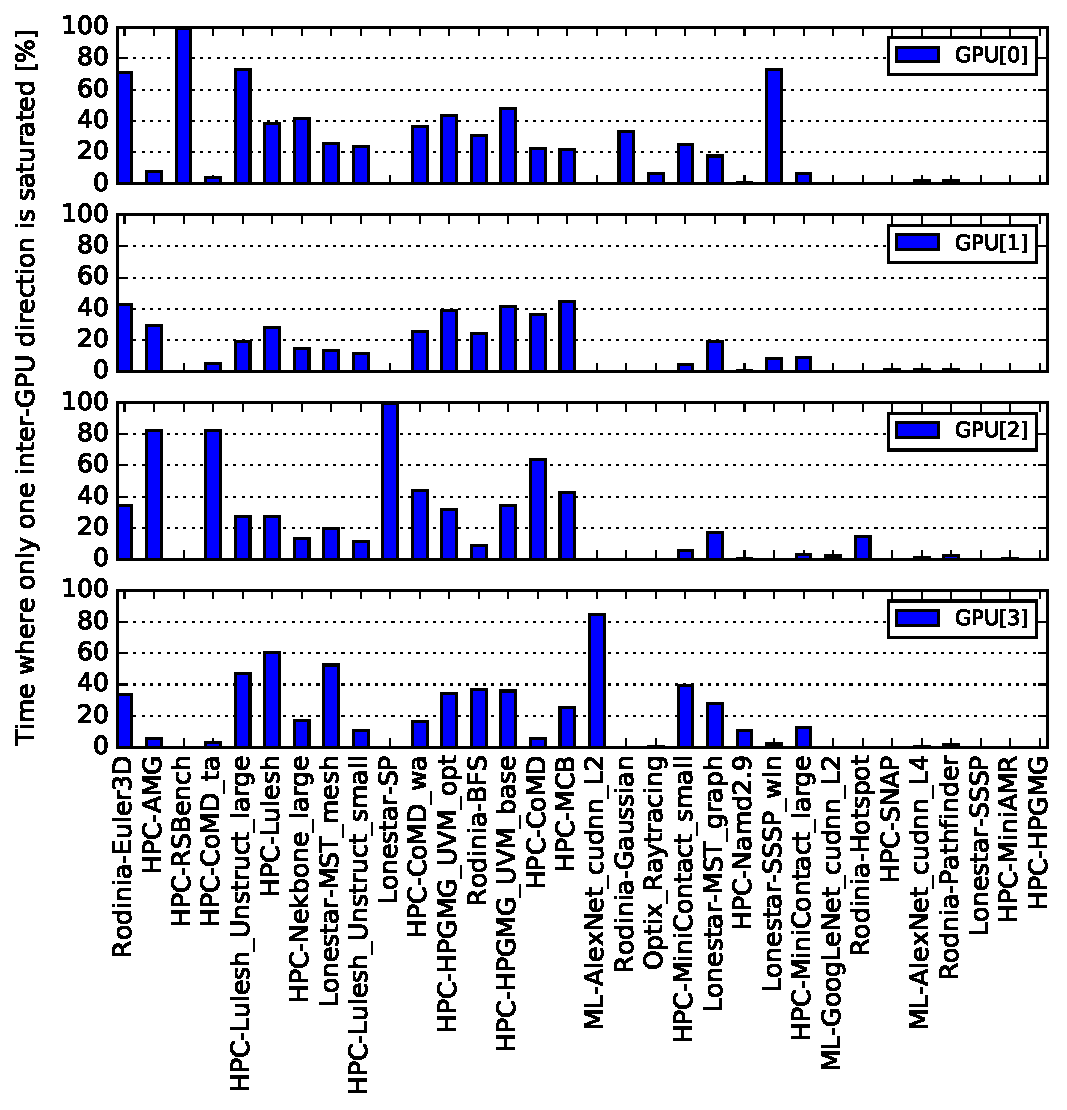
\includegraphics[width=0.9\columnwidth]{figures/plot_nvlink_chance.pdf}
=======
    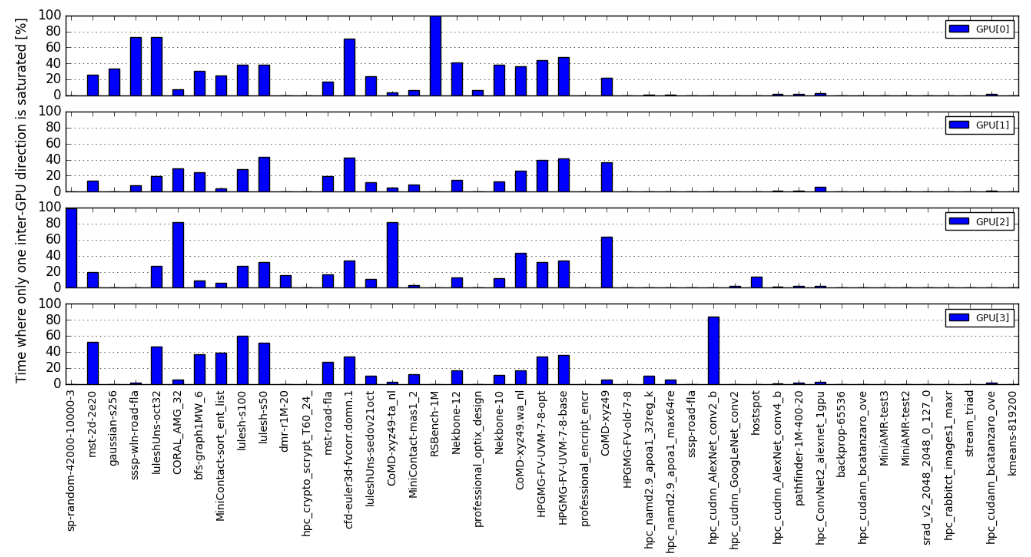
\includegraphics[width=1.0\columnwidth]{figures/link-motivation.jpg}
>>>>>>> 55401a9e4a1a10b4a8c8192a14d5f01dd9e642c1
    \caption{Maybe not exact right plot but show why there is room for 
improvement even in a normal link system.}
    \label{fig:link-motivation}
\end{figure}


\begin{figure*}[tp]
    \centering
<<<<<<< HEAD
    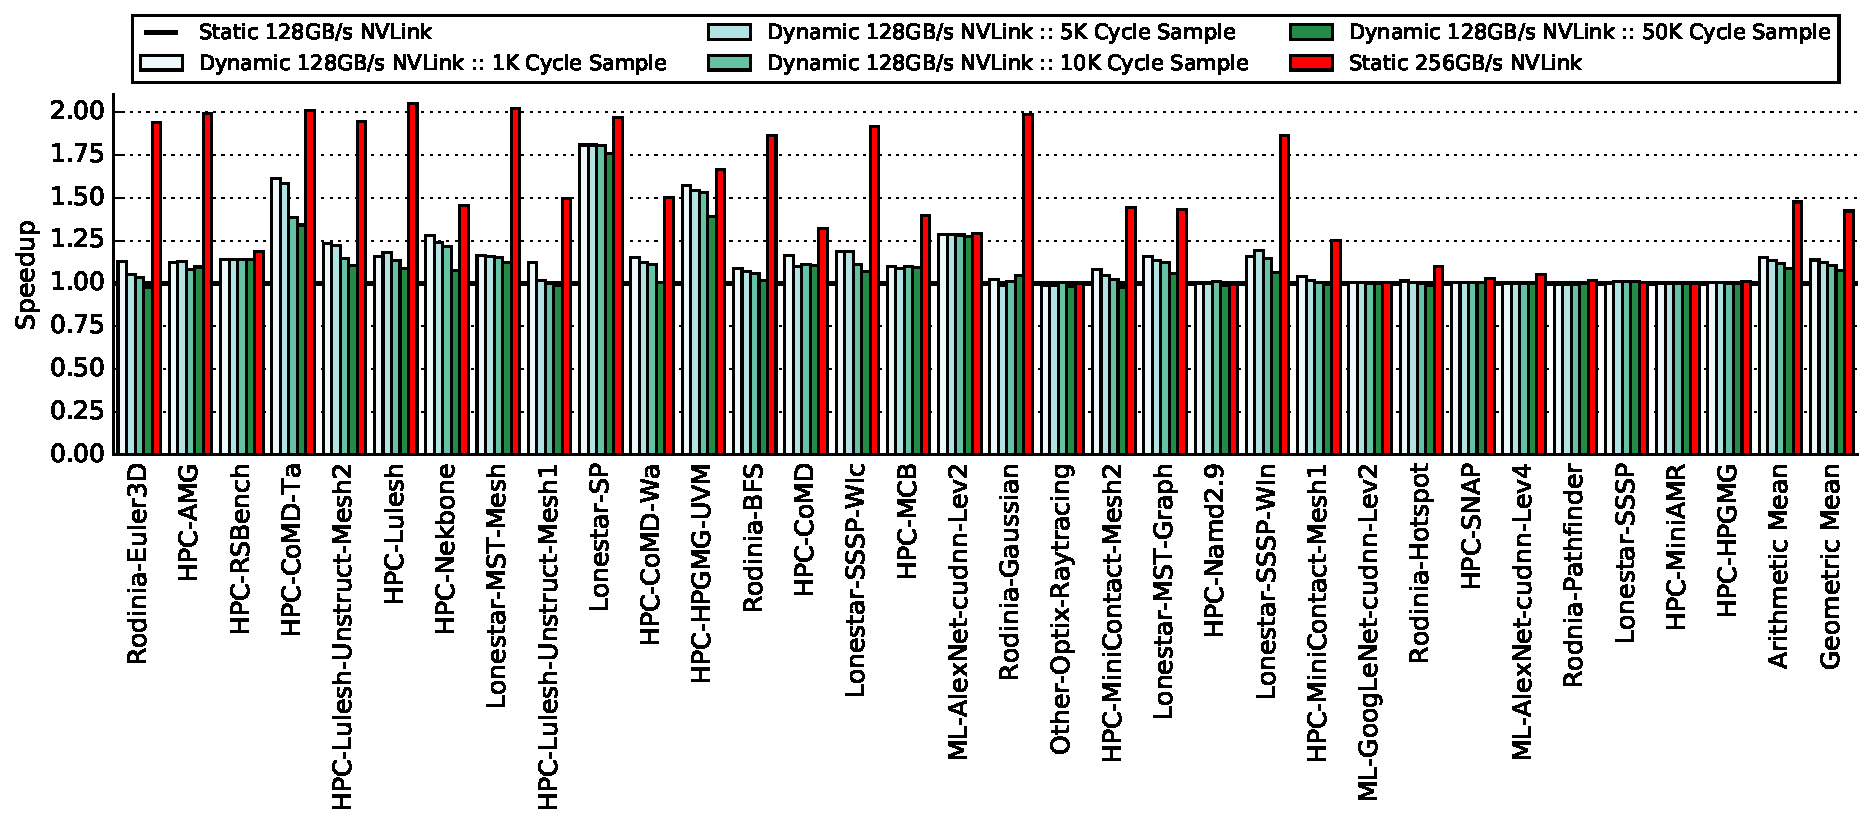
\includegraphics[width=0.9\textwidth]{figures/plot_nvlink_sample_time.pdf}
=======
    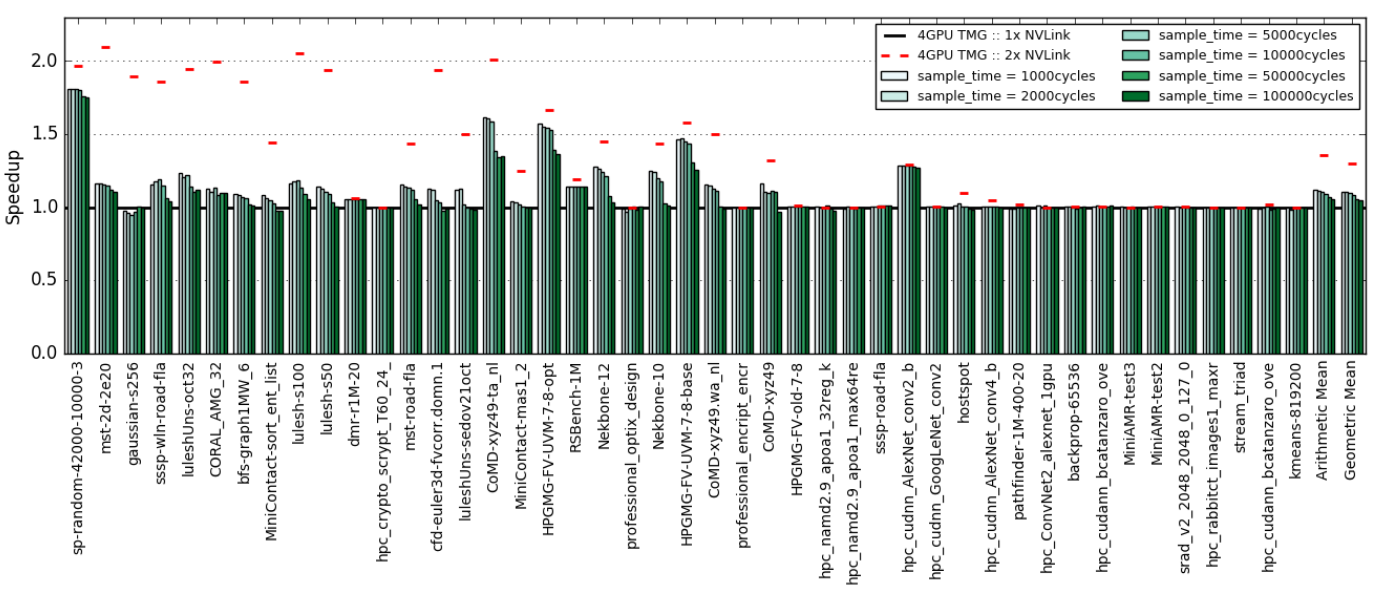
\includegraphics[width=1.0\textwidth]{figures/sample-time.jpg}
>>>>>>> 55401a9e4a1a10b4a8c8192a14d5f01dd9e642c1
    \caption{Show that we can adapt to application phasing without too many 
issues}
    \label{fig:sampletime}
\end{figure*}


\begin{figure*}[tp]
    \centering
<<<<<<< HEAD
    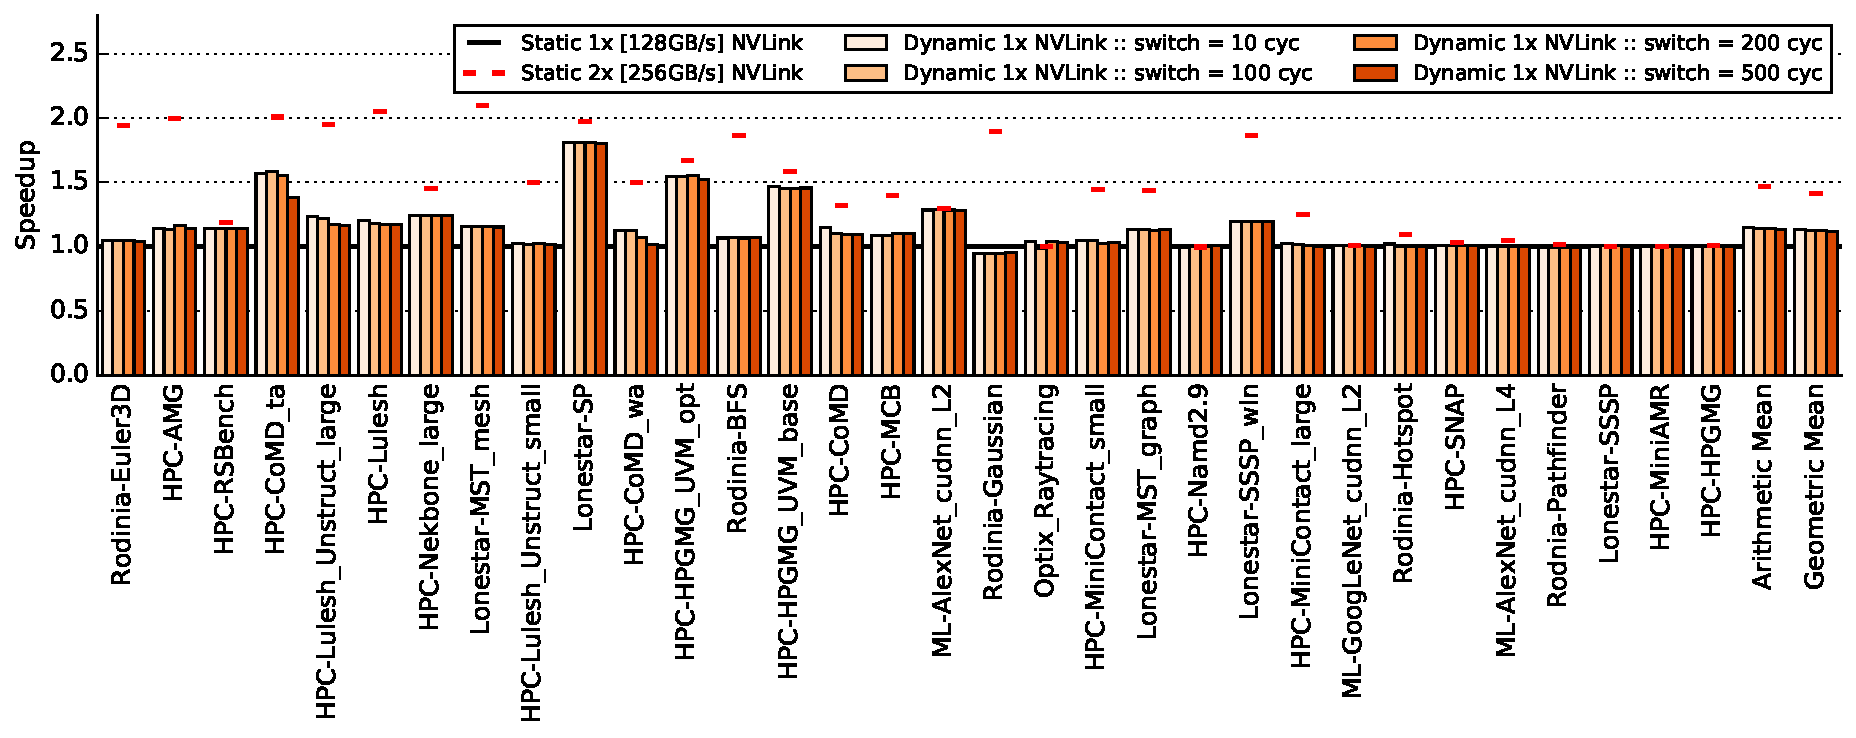
\includegraphics[width=0.9\textwidth]{figures/plot_nvlink_switch_time_sample_time5000.pdf}
=======
    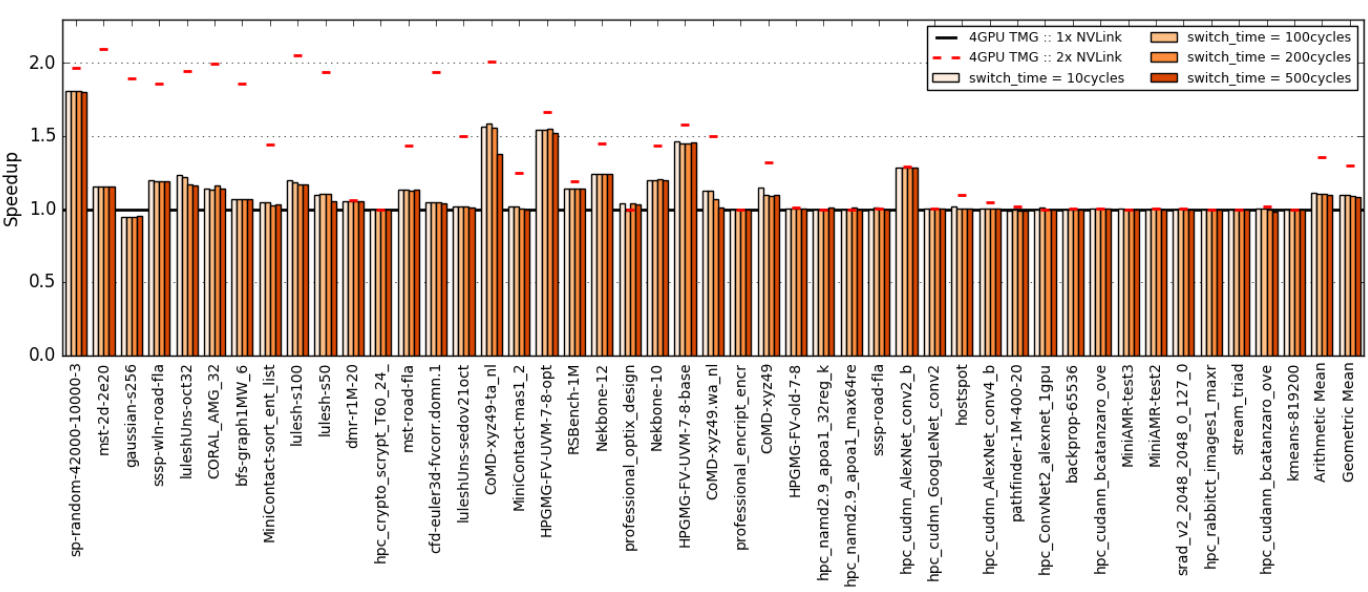
\includegraphics[width=1.0\textwidth]{figures/switch-time.jpg}
>>>>>>> 55401a9e4a1a10b4a8c8192a14d5f01dd9e642c1
    \caption{Show that when we're using a reasonable sample time like even 5k 
cycles, switch time is largely irrelevant.}
    \label{fig:switchtime}
\end{figure*}

\subsubsection{Results}
Results here